\section{Experiments}
In this section, we first evaluate our model on various downstream tasks, demonstrating its versatile decoding capabilities. Next, we assess its generalizability to novel subjects and its adaptability to real-world applications. Finally, we analyze the functions of queries in our neuroscience-informed attention mechanism.

\subsection{Settings}

\noindent\textbf{fMRI Datasets} 
We use the widely used Natural Scenes Dataset (NSD) \cite{allen2022massive}, a large-scale dataset consisting of fMRI measurements of $8$ healthy adult subjects. During data collection, subjects viewed images from the MS-COCO dataset \cite{lin2014microsoft} and were instructed to press buttons to indicate whether they had previously seen each image.

% \textit{Instruction datasets}
% COCO Caption \cite{chen2015microsoft}, Paragraph Captioning \cite{krause2017hierarchical},
% COCO QA \cite{ren2015exploring}, 
% VQAv2 \cite{goyal2017making}, Visual Genome \cite{krishna2017visual}, A-OKVQA \cite{schwenk2022okvqa}, ST-VQA \cite{biten2019scene}, OK-VQA \cite{marino2019ok}, \cite{acharya2019tallyqa}, VQA-E \cite{li2018vqa}, FSVQA \cite{shin2016color}
% VisDial \cite{murahari2019improving},
% LVIS-instruct4v \cite{wang2023see}, LLaVA Instruct 150K \cite{liu2023visual}

\noindent\textbf{Downstream Datasets} The downstream dataset will be discussed within each experiment section. See examples and a short description for all datasets we will use in Appendix~\ref {app:dataset}.
Implementation details could be found in Appendix~\ref{app:impl}.

\begingroup
\sisetup{
  table-format=3.2,  % 3 digits before the decimal, 2 after
  table-align-text-pre=false,
  propagate-math-font=true,
  table-number-alignment=center,
  detect-weight=true,detect-inline-weight=math
}
\def\Uline#1{#1\llap{\uline{\phantom{#1}}}}
\begin{table*}[t]\centering
% \vspace{-1em}
\caption{Versatile decoding. A dash $-$ means the model could not perform this task. The superscript $^\circ$ means the model is trained from scratch, in contrast to their BIT version. The CIDEr metric is scaled by a factor of 100 for consistency with Table~\ref{tab:caption} and baselines.}
\vskip 0.1in
\label{tab:versatile}
\resizebox{\linewidth}{!}{
\begin{tabular}{cc|SSS|SSS|SSS}\toprule
& & {OneLLM} & {UMBRAE} &{BrainChat} & {MindBridge$^\circ$} & {UniBrain$^\circ$} & {\makecell{\mindllm{}}$^\circ$} &{MindBridge} & {UniBrain} & {\makecell{\mindllm{}}} \\
\midrule
subj-agnostic &  & {\xmark}& {\xmark} & {\xmark} & {\cmark} & {\cmark} & {\cmark} &{\cmark} & {\cmark} & {\cmark} \\
% subj-agnostic &  & {\xmark}& {\xmark} & {\xmark} & {\xmark} & {\cmark} & {\cmark} &\xmark & {\cmark} & {\cmark} \\
\midrule
COCO-QA &Accuracy$\uparrow$ &11.09\% & 22.23\% & 39.44\% &40.19\% &38.38\% &42.09\% &\Uline{45.33\%} &42.00\% & \bfseries 48.19\% \\
\midrule
VG-QA &Accuracy$\uparrow$ & 8.76\% & 19.67\% & 21.00\% &20.84\% &21.27\% &21.68\% &23.53\% & \Uline{24.02\%} &\bfseries 24.06\% \\
\midrule
VQA-v2 &Accuracy $\uparrow$& 33.68\% & \Uline{51.23}\% & 40.02\% &43.25\% &46.04\% &44.13\% &47.91\% &48.58\% &\bfseries 52.14\% \\
\midrule
A-OKVQA &Accuracy $\uparrow$&25.23\%& 43.24\% &20.52\% &22.12\% &19.47\% &29.20\% & \Uline{50.44\%} &43.36\% &\bfseries 52.21\% \\
\midrule
ST-VQA &ANLS $\uparrow$& 5.74\%& 5.46\% &9.58\% &10.20\% &7.01\% &\Uline{12.76}\% &11.64\% &8.76\% &\bfseries 12.92\% \\
\midrule
OK-VQA &Accuracy $\uparrow$&22.98\% & 10.35\% &17.22\%&27.63\% &18.63\% &27.70\% &32.13\% &\Uline{32.30\%} & \bfseries 33.33\% \\
\midrule
\multirow{2}{*}{TallyQA} &Accuracy $\uparrow$& 8.34\% & 44.10\% & 43.22\%&43.49\% &44.83\% &43.75\% &49.46\% & \Uline{53.77\%} &\bfseries 54.76\% \\
&RMSE $\downarrow$&7.45 & 3.94 & 1.90 &2.03 &1.83 &2.04 &1.86 &\bfseries 1.67 &\Uline{1.76} \\
\midrule
\multirow{6}{*}{Paragraph Caption} &BLEU-1$\uparrow$ &0.26 & \bfseries 29.82 & 22.21&21.82 &25.69 &26.49 &25.69 &28.28 & \Uline{29.43} \\
&BLEU-2 $\uparrow$ &0.08 & 14.26 &10.23 &10.47 &12.62 &12.48 &13.00 &\Uline{15.47} & \bfseries 15.78 \\
&BLEU-3$\uparrow$ &0.03 & 6.52 &6.38 &5.58 &6.70 &6.43 &7.10 &\Uline{8.90} & \bfseries 9.14 \\
&BLEU-4$\uparrow$ &0.01 & 2.95 &2.12 &3.14 &3.81 &3.63 &4.22 &\bfseries5.60 & \Uline{5.51} \\
&METEOR $\uparrow$&2.36 &12.60 &9.10 &10.95 &11.13 &10.71 &11.39 &\bfseries13.50 & \Uline{13.18} \\
&CIDEr $\uparrow$&0.00 & 7.39 &6.02& \Uline{7.50} &3.92 &2.44 & 3.55 &1.82 & \bfseries 7.80 \\
\midrule
\multirow{8}{*}{VQA-E} &Accuracy $\uparrow$ &19.60\%& 47.84\% &46.20\% &45.40\% &44.42\% &44.55\% &\Uline{48.48\%} &48.39\% &\bfseries 50.95\% \\
&BLEU-1 $\uparrow$&17.32& 29.83 & 35.99 &35.63 &35.30 &35.08 &36.18 &\Uline{37.26} &\bfseries 37.70 \\
&BLEU-2 $\uparrow$&7.44& 14.76 & 18.33  &18.27 &18.04 &17.82 &19.38 &\Uline{20.41} &\bfseries 20.56 \\
&BLEU-3 $\uparrow$&3.62& 8.17 & 10.01 &10.32 &10.20 &10.05 &11.30 &\Uline{12.25} &\bfseries 12.34 \\
&BLEU-4 $\uparrow$&1.82& 4.87 &6.60 &6.27 &6.14 &6.00 &7.00 &\Uline{7.83} &\bfseries 7.92 \\
&CIDEr $\uparrow$&19.32& 63.26 &78.33 &79.05 &77.31 &76.80 &86.62 &\Uline{92.09} & \bfseries 93.60 \\
&METEOR $\uparrow$&6.69 & 12.25 &13.64 &14.13 &13.89 &13.96 &14.81 &\Uline{15.51} &\bfseries 15.62 \\
&ROUGE $\uparrow$&16.84& 28.38 & 32.82&33.78 &33.25 &33.11 &34.56 &\Uline{35.87} &\bfseries 35.88 \\
\midrule
\multirow{8}{*}{FSVQA} &VQA Acc. $\uparrow$& 31.44\% & 40.67\% &36.30\% &42.00\% &37.05\% &42.53\% &\Uline{45.95\%} &44.58\% &\bfseries 48.03\% \\
&FSVQA Acc. $\uparrow$& 21.02\% & 0.00\% & 30.22\% &37.40\% &32.30\% &38.50\% &\Uline{40.97\%} &37.87\% &\bfseries 43.00\% \\
&BLEU-1 $\uparrow$& 37.42 & 23.11 & 83.99&85.68 &83.84 &85.88 &\Uline{86.52} &85.10 &\bfseries 87.10 \\
&BLEU-2 $\uparrow$ & 31.72 & 5.86&78.50 &81.27 &78.81 &81.62 &\Uline{82.28} &80.01 &\bfseries 83.03 \\
&BLEU-3 $\uparrow$& 26.95 & 2.10&73.00 &77.10 &73.97 &77.62 &\Uline{78.34} &75.49 &\bfseries 79.27 \\
&BLEU-4 $\uparrow$& 22.48 & 1.04 &69.73 &72.89 &68.91 &73.56 &\Uline{74.35} &70.73 &\bfseries 75.50 \\
&METEOR $\uparrow$& 26.35 & 8.93 &44.76 &47.59 &45.94 &47.96 &\Uline{48.63} &46.89 &\bfseries 49.05 \\
&CIDEr $\uparrow$& 312.75 & 4.07 &600.00 &636.40 &609.00 &646.26 &\Uline{657.02} &628.83 &\bfseries 666.26 \\
\midrule
\multirow{8}{*}{Previous Caption} & BLEU-1 $\uparrow$ & 41.86  & {$-$} & 21.19 & 21.17 & 24.84 & \Uline{44.52} & 42.45 & 43.01 & \bfseries 47.20 \\
&BLEU-2 $\uparrow$ & 19.44 & {$-$} & 8.00 & 7.57 & 9.70 & \Uline{22.46} & 20.04 & 20.03 & \bfseries 25.16\\
&BLEU-3 $\uparrow$ & 9.25 & {$-$} & 1.98 & 2.85 & 3.40 & \Uline{10.39} & 9.61 & 9.19 & \bfseries 12.95\\
&BLEU-4 $\uparrow$ & 3.67 & {$-$} & 1.02& 1.28 & 1.46 & \Uline{5.45} &  5.31 & 4.58 & \bfseries 7.49 \\
&METEOR $\uparrow$ & 10.14 & {$-$} & 6.55& 6.46 & 7.20 & \Uline{11.00} & 10.83 & 10.81 & \bfseries 11.96 \\
&ROUGE $\uparrow$ & 30.19 & {$-$} & 21.23& 20.88 & 23.04 & \Uline{33.20} &32.38 & 31.99 & \bfseries 34.58 \\
&CIDEr $\uparrow$ & 6.65 & {$-$} & 9.21& 8.83 & \Uline{11.73} & 9.39 & 7.89 & 7.53 & \bfseries 16.02 \\
&SPICE $\uparrow$ & 2.49 & {$-$} & 2.44& 2.56 & 2.78 & \Uline{3.07} & 2.80 & 2.92 & \bfseries 3.93 \\
\bottomrule
\end{tabular}}
% \vspace{-1em}
\end{table*}
\endgroup

\subsection{Brain Captioning}
To evaluate the model's performance on downstream tasks, we start with the widely used brain captioning benchmark \cite{xia2024umbrae}. The task, built upon COCO Caption \cite{chen2015microsoft} requires the model to predict captions of given images as fMRI stimuli.

\noindent\textbf{Baselines}
The following baselines are considered in this experiment: SDRecon \cite{takagi2023high}, UniBrain \cite{mai2023unibrain}, and BrainCap \cite{ferrante2023brain} employs a linear regression, mapping the fMRI to the inputs of an image caption model \cite{li2023blip}. OneLLM \cite{han2024onellm} is a multimodal large language models that align $8$ modalities (including fMRI) with language all in one model. For fair and efficient comparison, we only finetune the encoder, given that we freeze the LLM in our method as well. UMBRAE learns an encoder that maps fMRIs to images through an encoder similar to the MLP mixer \cite{tolstikhin2021mlp}. BrainChat \cite{huang2024brainchat} segments the flattened voxels into 16 patches and employs a transformer to decode text conditioned on the patches.
It is worth noting that all of these baselines require subject-specific layers or parameters. In contrast, our model is subject-agnostic, thus with the potential to generalize on novel subjects.

\noindent\textbf{Metric} Following previous works, we use five standard metrics for text generation: BLEU-$k$ \cite{papineni2002bleu}, ROUGE-L \cite{lin2004rouge}, CIDEr \cite{vedantam2015cider}, SPICE \cite{anderson2016spice}, METEOR \cite{banerjee2005meteor}.

Table \ref{tab:caption} shows that our model outperforms baselines in terms of most metrics, with an average improvement of $3.32\%$, even if our model does not have any subject-specific layers. We argue that this is attributed to both the novel architecture design and the introduction of BIT, which will be evident in the next experiment.

\begingroup
\sisetup{
  table-format=3.2,  % 3 digits before the decimal, 2 after
  table-align-text-pre=false,
  table-number-alignment=center,
detect-weight=true,detect-inline-weight=math
}
\begin{table}[t]
\vspace{-1em}
\centering
\caption{Model generalization, compared with subject-agnostic model. We train the models on subject $1-7$ and evaluate on subject $8$, which is the held-out subject.}
\label{tab:subj8}
\vskip 0.1in

\resizebox{\linewidth}{!}{
\begin{tabular}{ccSSS}\toprule
& & {MindBridge} & {UniBrain} & {\mindllm{}} \\
\midrule
COCO-QA &Accuracy $\uparrow$&35.88 &24.95 &\bfseries 38.96 \\
\midrule
VG-QA &Accuracy $\uparrow$&\bfseries 20.56 &16.23 & 19.29 \\
\midrule
VQA-v2 &Accuracy $\uparrow$&42.80 &40.16 &\bfseries 46.04 \\
\midrule
A-OKVQA &Accuracy $\uparrow$&44.55 &28.71 &\bfseries 45.54 \\
\midrule
ST-VQA &ANLS $\uparrow$&9.33 &9.30 &\bfseries 13.63 \\
\midrule
OK-VQA &Accuracy $\uparrow$&21.94 &17.09 &\bfseries 25.44 \\
\midrule
\multirow{2}{*}{TallyQA} &Accuracy $\uparrow$&38.92 &32.51 &\bfseries 42.29 \\
&RMSE $\downarrow$&2.12 &\bfseries 2.02 & 2.11 \\
\midrule
\multirow{8}{*}{COCO-Caption} &BLEU-1 $\uparrow$&39.84 &41.90 &\bfseries 44.60 \\
&BLEU-2 $\uparrow$&19.55 &19.67 &\bfseries 24.04 \\
&BLEU-3 $\uparrow$&9.29 &8.89 &\bfseries 12.79 \\
&BLEU-4 $\uparrow$&5.24 &4.33 &\bfseries 7.52\\
&METEOR $\uparrow$&10.39 &10.80 &\bfseries 11.16 \\
&ROUGE $\uparrow$&31.10 &31.54 &\bfseries 33.47 \\
&CIDEr $\uparrow$& 8.70 &6.40 & \bfseries 13.22 \\
&SPICE $\uparrow$&2.67 &2.39 &\bfseries 3.82 \\
\midrule
\multirow{6}{*}{Paragraph Caption} &BLEU-1 $\uparrow$&23.18 &21.73 &\bfseries 26.07 \\
&BLEU-2 $\uparrow$&10.71 &8.94 &\bfseries 12.64 \\
&BLEU-3 $\uparrow$&4.61 &3.72 &\bfseries 6.27 \\
&BLEU-4 $\uparrow$&2.22 &1.92 &\bfseries 3.46 \\
&METEOR $\uparrow$&9.99 &9.47 &\bfseries 11.18 \\
&CIDEr $\uparrow$&0.71 &1.56 &\bfseries 5.61 \\
\midrule
\multirow{8}{*}{VQA-E} &Accuracy $\uparrow$&41.78 &38.53 &\bfseries 46.19 \\
&BLEU-1 $\uparrow$&32.54 &32.86 &\bfseries 34.54 \\
&BLEU-2 $\uparrow$&16.13 &15.48 &\bfseries 17.54 \\
&BLEU-3 $\uparrow$&8.82 &7.98 &\bfseries 9.84 \\
&BLEU-4 $\uparrow$&5.16 &4.42 &\bfseries 5.81 \\
&CIDEr $\uparrow$&68.13 &58.79 &\bfseries 73.27 \\
&METEOR $\uparrow$&12.74 &12.26 &\bfseries 13.56 \\
&ROUGE $\uparrow$&30.63 &29.38 &\bfseries 32.36 \\
\midrule
\multirow{8}{*}{FSVQA} &VQA Acc. $\uparrow$&42.33 &37.92 &\bfseries 43.92 \\
&FSVQA Acc. $\uparrow$&37.16 &30.83 &\bfseries 39.07 \\
&BLEU-1 $\uparrow$&75.81 &82.94 &\bfseries 86.19 \\
&BLEU-2 $\uparrow$&71.03 &77.24 &\bfseries 81.83 \\
&BLEU-3 $\uparrow$&66.40 &71.94 &\bfseries 77.77 \\
&BLEU-4 $\uparrow$&61.55 &66.54 &\bfseries 73.58 \\
&METEOR $\uparrow$&45.84 &45.24 &\bfseries 47.94 \\
&CIDEr $\uparrow$&428.39 &587.78 &\bfseries 646.30 \\
\bottomrule
\end{tabular}
}
\vspace{-1em}
\end{table}
\endgroup

\subsection{Versatile Decoding}
The purpose of experiments in this section is two-fold: 1) To investigate the impact of our model design and the introduction of BIT on performance improvement. 2) To evaluate the versatility of the model, i.e., its performance on various downstream tasks.

\noindent\textbf{Baselines} Besides baselines that could be adapted to this experiment from the previous one, we further consider the following subject-agnostic models as baselines.
1) MindBridge \cite{wang2024mindbridge} flattens the voxels and adaptively adjusts the padding and stride to pool the voxels into a fixed dimension. The original implementation of MindBridge has subject-specific parameters. However, since those parameters are of the same size, we make them shared across subjects and thus make the model subject-agnostic.
2) UniBrain \cite{wang2024unibrain} samples voxels into a fixed number of groups and employs a transformer where groups are treated as tokens. This UniBrain is unrelated to the UniBrain in the previous section; they just share the same name.

\noindent\textbf{Datasets \& Metric}
We use the test split of all QA \& caption datasets in the BIT dataset. We strictly adhere to the official metrics on all datasets. In summary, for sentence generation, we use BLEU-$k$~\cite{papineni2002bleu}, ROUGE-L~\cite{lin2004rouge}, CIDEr~\cite{vedantam2015cider}, SPICE~\cite{anderson2016spice}, METEOR~\cite{banerjee2005meteor}. For QA-related tasks, we use VQA accuracy~\cite{antol2015vqa} as well as special metrics proposed in the original paper (e.g. ANLS for ST-VQA~\cite{biten2019scene}).

The results on subject 1 are shown in Table~\ref{tab:versatile}. Our model outperforms baselines, with an average improvement of $12.0\%$. Further, by comparing instruction tuning and from-scratch models, we find that instruction tuning has a significant positive effect, with an average improvement of $28.0\%$. The results remain stable across different random seeds; for instance, according to our observations, the BLEU-1 score for paragraph captioning exhibits a maximum of $\pm 0.3$ variance. We report experiments on other subjects in Appendix~\ref{app:breakdown}.

\begingroup
\sisetup{
  table-format=2.2,  % 3 digits before the decimal, 2 after
  table-align-text-pre=false,
  table-number-alignment=center,
detect-weight=true,detect-inline-weight=math
}
\begin{table}[htbp]
% \vspace{-1.5em}
    \caption{Model adaptation to new tasks. \textit{sentiment understanding} and \textit{utility/affordance} are sub-datasets from TDIUC that are particularly relevant to BCI applications.}
    \label{tab:new_task}
\vskip 0.1in
    \centering
    \resizebox{\linewidth}{!}{
    \begin{tabular}{cSSSS}
    \toprule
    \multirow{2}{*}{Method} &  \multicolumn{2}{c}{Overall} & {Sentiment Understanding} & {Utility/Affordance} \\
    \cmidrule{2-3} \cmidrule{4-4} \cmidrule{5-5}
    & {A-MPT} & {H-MPT} & {Accuracy} & {Accuracy} \\
    \midrule
    \mindllm{}$^\circ$ & 41.09\% & 19.38\% & 70.00\% & 0.00\%\\
    \midrule
         MindBridge & 49.77\% & 39.88\% & 80.00\% & 14.29\%\\
         UniBrain & 51.50\% & 36.76\% & 80.00\% & 28.57\%\\
         \mindllm{}& \bfseries 54.08\% &  \bfseries 45.43\% & \bfseries 80.77\% & \bfseries 50.00\% \\
    \bottomrule
    \end{tabular}
    }
    \vspace{-1em}
\end{table}
\endgroup


\subsection{Unseen Subject Generalization}
Our neuroscience-informed, subject-agnostic design enhances generalization to novel subjects, a crucial factor in real-world applications where training a model for each individual is impractical. To evaluate it, we perform instruction tuning on $7$ out of the $8$ subjects in the natural scene dataset \cite{allen2022massive}, and evaluate generalization on the held-out subject. Table~\ref{tab:subj8} shows our model outperforms two other subject-agnostic baselines in most cases, with an average improvement of $24.5\%$ compared to the second-best model. We anticipate further performance gains through the application of domain adaptation techniques \cite{xiao2023spa,ganin2015unsupervised,ganin2016domain,gong2012geodesic}, which we leave as a direction for future work.

\subsection{Adapting to New Tasks}
It is common that users want to adapt the \mindllm{} to their own specific use cases. To this end, we aim to assess our model's adaptability to new tasks.

\noindent\textbf{Dataset \& Metrics} We use TDIUC \cite{kafle2017analysis}, a QA dataset consisting of $12$ types of questions, as a benchmark to evaluate the model's various capabilities comprehensively. Additionally, we further select $2$ task types-\textit{sentiment understanding} and \textit{utility/affordance} tasks, that are particularly relevant to BCI applications as sub-datasets. The \textit{utility/affordance} task, for instance, enables the model to identify useful objects in a given scene and autonomously decide whether to utilize them. Following their paper, we compute the accuracy of each type and report the arithmetic mean-per-type (A-MPT) and the harmonic mean-per-type (H-MPT). For the $2$ selected types, we report the accuracy respectively. 

Table~\ref{tab:new_task} shows our model achieves balanced (high harmonic mean) and consistently improved performances with an average of $13.5\%$. We could also observe the performance benefits from BIT, with $25.0\%$ absolute improvement.

% \begin{figure*}[t]
%     \begin{subfigure}[c]{0.15\textwidth}
%         \centering
%         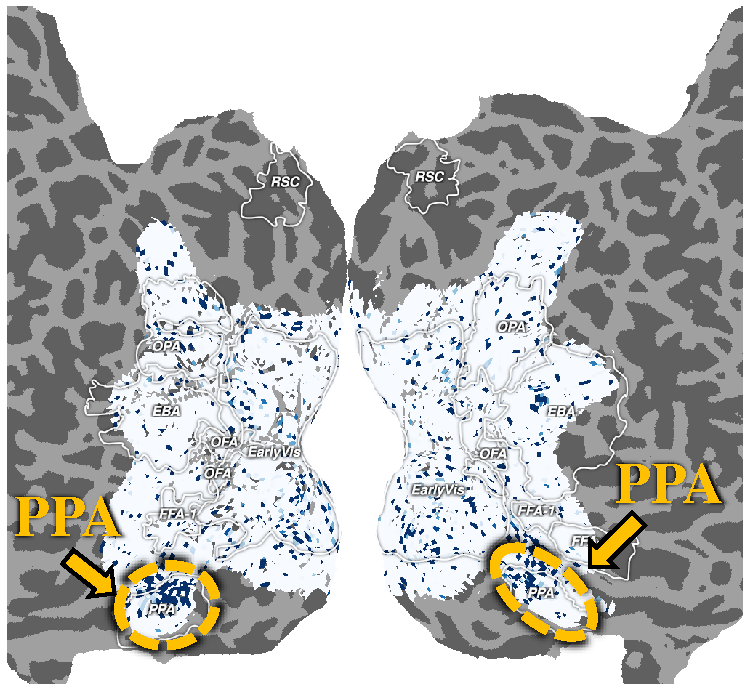
\includegraphics[width=\textwidth]{figures/brain_query/brain_query_ppa.pdf}
%         % \caption{Query: PPA}
%         \vspace{-1.5em}
%         \caption{}
%         \label{sub:ppa}
%     \end{subfigure}
%     \hfill
%     \begin{subfigure}[c]{0.15\textwidth}
%         \centering
%         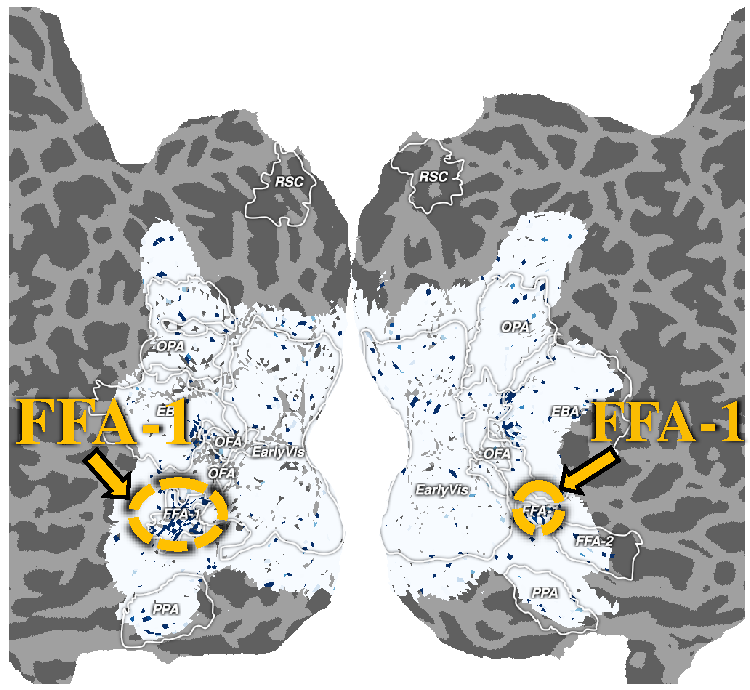
\includegraphics[width=\textwidth]{figures/brain_query/brain_query_ffa_1.pdf}
%         % \caption{Query: FFA-1}
%         \vspace{-1.5em}
%                 \caption{}
%         \label{sub:ffa-1}
%     \end{subfigure}
%     \hfill
%     \begin{subfigure}[c]{0.15\textwidth}
%         \centering
%         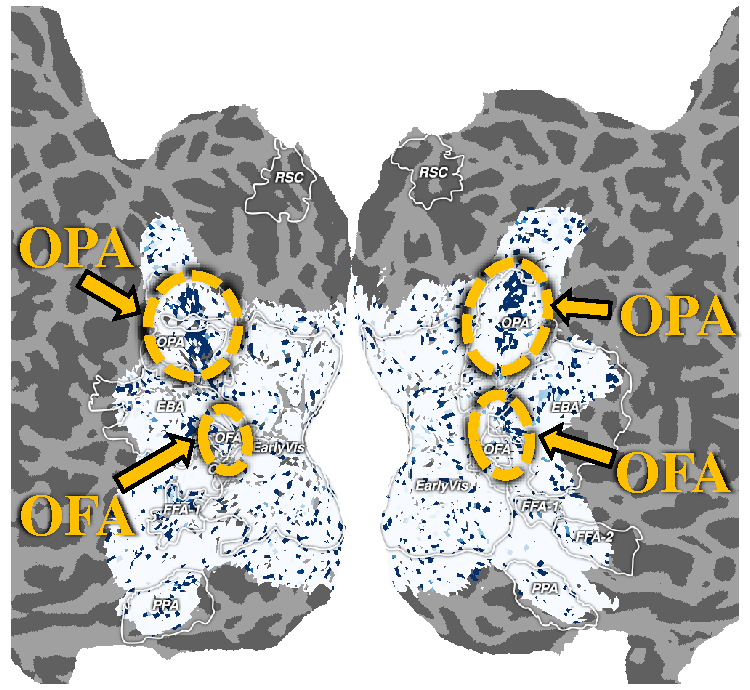
\includegraphics[width=\textwidth]{figures/brain_query/brain_query_opa_ofa.pdf}
%         % \caption{Query: FFA-1}
%         \vspace{-1.5em}
%         \caption{}
%         \label{sub:opa_ofa}
%     \end{subfigure}
%     \hfill
%     \begin{subfigure}[c]{0.15\textwidth}
%         \centering
%         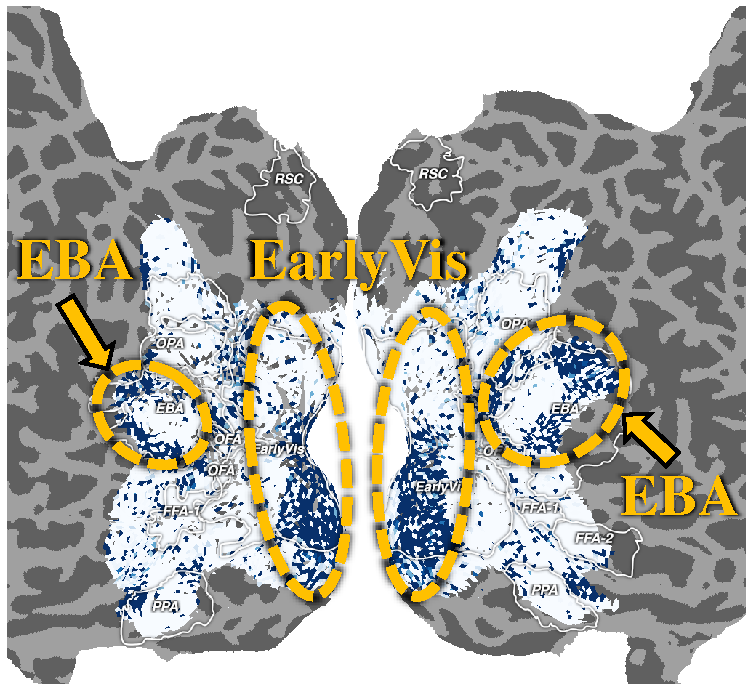
\includegraphics[width=\textwidth]{figures/brain_query/brain_query_earlyvis_eba.pdf}
%         % \caption{Query: FFA-1}
%         \vspace{-1.5em}
%         \caption{}
%         \label{sub:ev_eba}
%     \end{subfigure}
%     \hfill
%     \begin{subfigure}[c]{0.15\textwidth}
%         \centering
%         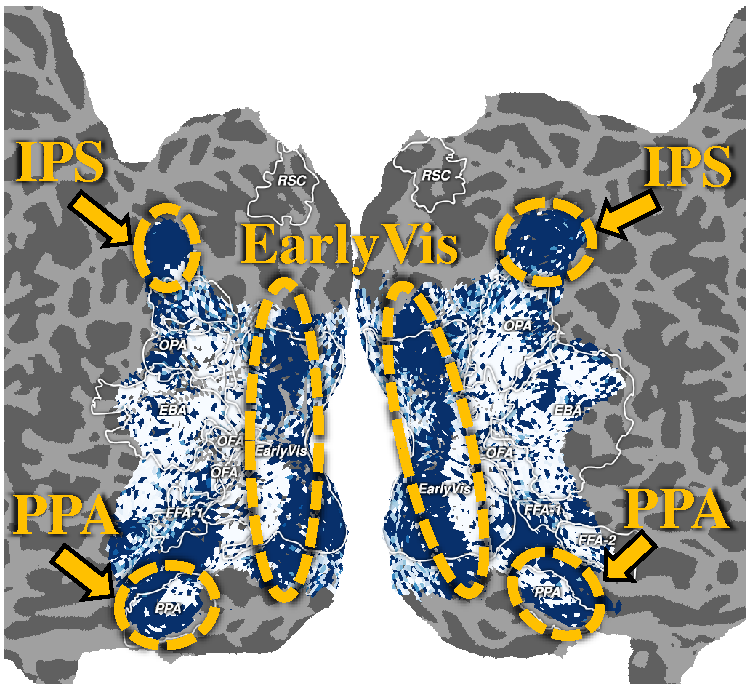
\includegraphics[width=\textwidth]{figures/brain_query/brain_query_multi_low_high.pdf}
%         % \caption{Query: FFA-1}
%         \vspace{-1.5em}
%         \caption{}
%         \label{sub:low_high}
%     \end{subfigure}
%     \hfill
%     \begin{subfigure}[c]{0.15\textwidth}
%         \centering
%         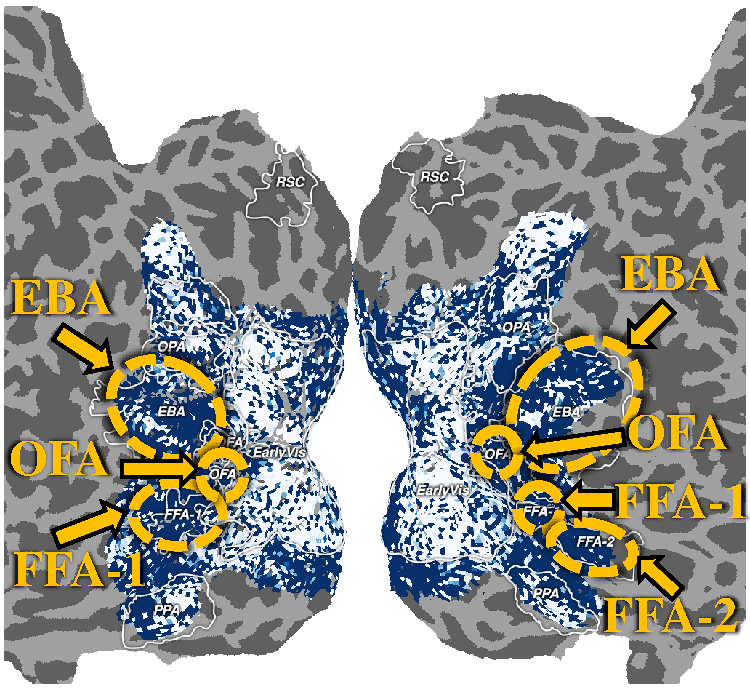
\includegraphics[width=\textwidth]{figures/brain_query/brain_query_multi_high_high.pdf}
%         % \caption{Query: FFA-1}
%         \vspace{-1.5em}
%         \caption{}
%         \label{sub:high_high}
%     \end{subfigure}
%     \hfill
%     \begin{subfigure}[c]{0.05\textwidth}
%         \centering
%         
\includegraphics[width=\textwidth]{figures/brain_query/colorbar.png}
%     \end{subfigure}
%     \vspace{-1.4em}
%     \caption{Visaulization of attention weights between \textit{queries} and brain voxels. Each subfigure represents a \textit{query} token, and the strength of color indicates its attention weight (after min-max normalization) to each voxel. 
%     }
%     \label{fig:query}
%     \vspace{-1.2em}
% \end{figure*}

\subsection{Performance scale with the number of subjects}

We conducted experiments to evaluate how model performance scales with the number of subjects and report performances on the COCO caption task. We examined both the in-distribution (seen subjects) setting in Figure~\ref{tab:in} and the out-of-distribution (held-out subjects) setting in Figure~\ref{tab:out}. Our results show significant performance improvements as the number of training subjects increases, demonstrating that the model benefits from exposure to more subjects during pre-training.

\begingroup
\sisetup{
  table-format=3.2,  % 3 digits before the decimal, 2 after
  table-align-text-pre=false,
  table-number-alignment=center,
detect-weight=true,detect-inline-weight=math
}
\begin{table}[!htp]\centering
\caption{Performance scaling with number of subjects (in-distribution). Evaluation is performed on Subject 1, who is included during training.}\label{tab:in}
\vskip 0.1in
\resizebox{\linewidth}{!}{
\begin{tabular}{cSSSSSSSSS}\toprule
& \multicolumn{8}{c}{COCO Caption}  \\
\makecell{number\\of\\subjects} &{{BLEU-1} $\uparrow$} & {BLEU-2 $\uparrow$} & {BLEU-3 $\uparrow$} & {{BLEU-4} $\uparrow$} &{METEOR $\uparrow$}&{ROUGE $\uparrow$}& {CIDEr $\uparrow$}&{SPICE $\uparrow$}\\
\midrule
1 &58.05 &37.95 &24.40 &16.14 &16.62 &42.03 &43.04 &8.81 \\
3 &56.81 &37.16 &24.12 &16.30 &16.44 &41.93 &40.94 &9.12 \\
5 &58.17 &38.65 &25.49 &17.30 &16.97 &42.36 &46.54 &9.19 \\
7 &58.52 &39.20 &25.95 &17.51 &17.12 &42.87 &47.45 &9.48 \\
\bottomrule
\end{tabular}
}
\end{table}

\begin{table}[!htp]\centering
\caption{Performance scaling with number of subjects (out-of-distribution). Evaluation is performed on Subject 8, who is held out during training.}\label{tab:out}
\vskip 0.1in
\resizebox{\linewidth}{!}{
\begin{tabular}{cSSSSSSSSS}\toprule
\makecell{number\\of\\subjects} &{{BLEU-1} $\uparrow$} & {BLEU-2 $\uparrow$} & {BLEU-3 $\uparrow$} & {{BLEU-4} $\uparrow$} &{METEOR $\uparrow$}&{ROUGE $\uparrow$}& {CIDEr $\uparrow$}&{SPICE $\uparrow$}\\
\midrule
1 &42.40 &19.51 &8.61 &4.19 &9.48 &30.68 &5.41 &1.70 \\
3 &43.95 &22.45 &10.37 &5.53 &10.37 &32.49 &5.79 &2.59 \\
5 &45.00 &22.61 &10.64 &5.60 &10.53 &32.53 &6.22 &2.79 \\
7 &47.30 &25.35 &13.61 &8.15 &11.40 &34.64 &6.41 &3.61 \\
\bottomrule
\end{tabular}
} 
\end{table}

\endgroup


\subsection{Ablation Study}
We conduct ablation studies on the design of key embeddings in the neuroscience-informed attention module in Figure~\ref{fig:ablation}. The results strongly validate our design. The vanilla cross attention (\textit{Pos Enc.+fMRI}) leads to poor performance, while removing fMRI values from the key embeddings (\textit{Pos Enc.}) yields a significant improvement. Replacing positional encoding with region encodings (\textit{Reg. Enc.}) accelerates convergence in the early stages since it is grounded by neuroscientific principles. However, it is eventually outperformed by \textit{Pos Enc.} due to the lack of finer-grained information. Combining the positional encoding and region encodings (\textit{Pos Enc.+Reg Enc.}) achieves the best model design. In addition, replacing positional encoding with an MLP that maps coordinates to embeddings results in poor performance (\textit{(x,y,z)+MLP}), which indicates the amount of high-frequency spatial information in fMRI signals. Additional ablation results on evaluation metrics are provided in Appendix~\ref{app:ablation}.

\begin{figure}[h]
% \vspace{-0.8em}
    \centering
    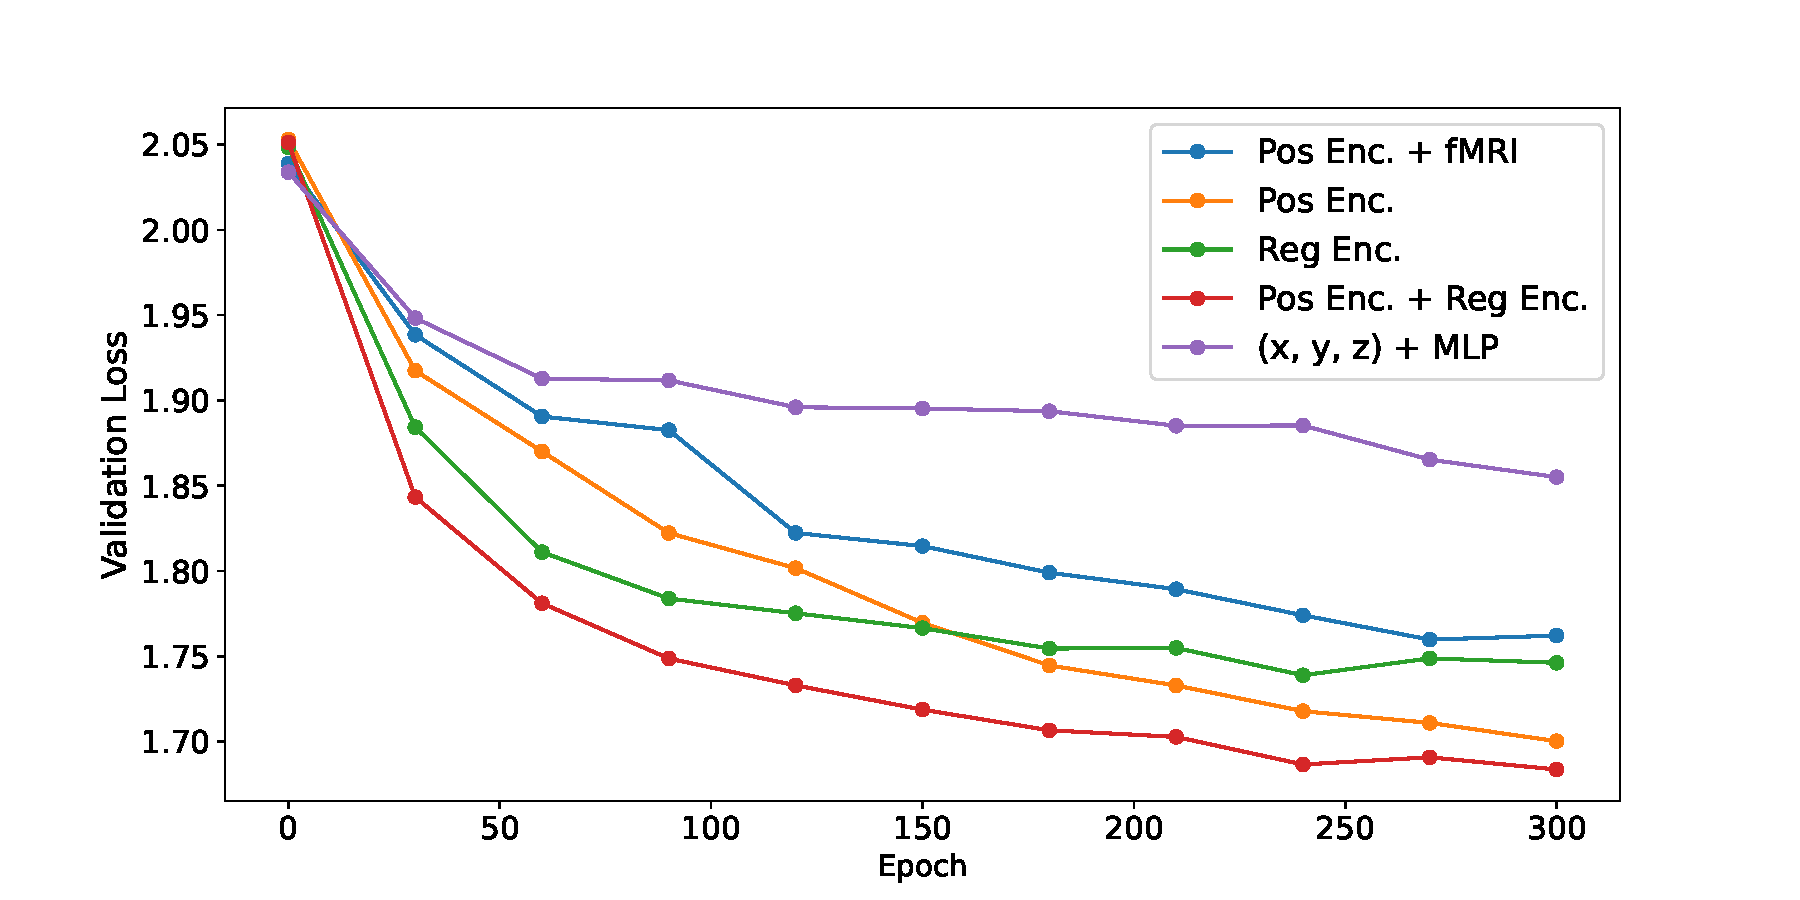
\includegraphics[width=\linewidth]{figures/ablation.pdf}
    \vspace{-2em}
    \caption{Ablation study of the key embedding design. Pos Enc. stands for positional encoding. Reg Enc. stands for multiple region encodings. \textit{(x, y, z)+MLP} means we employ an MLP to map the coordinates to the embeddings instead of positional encoding.}
    \label{fig:ablation}
    % \vspace{-1.3em}
\end{figure}
\subsection{Visualizations and Interpretations}
\label{sec:vis}

\begin{figure}
    \centering
    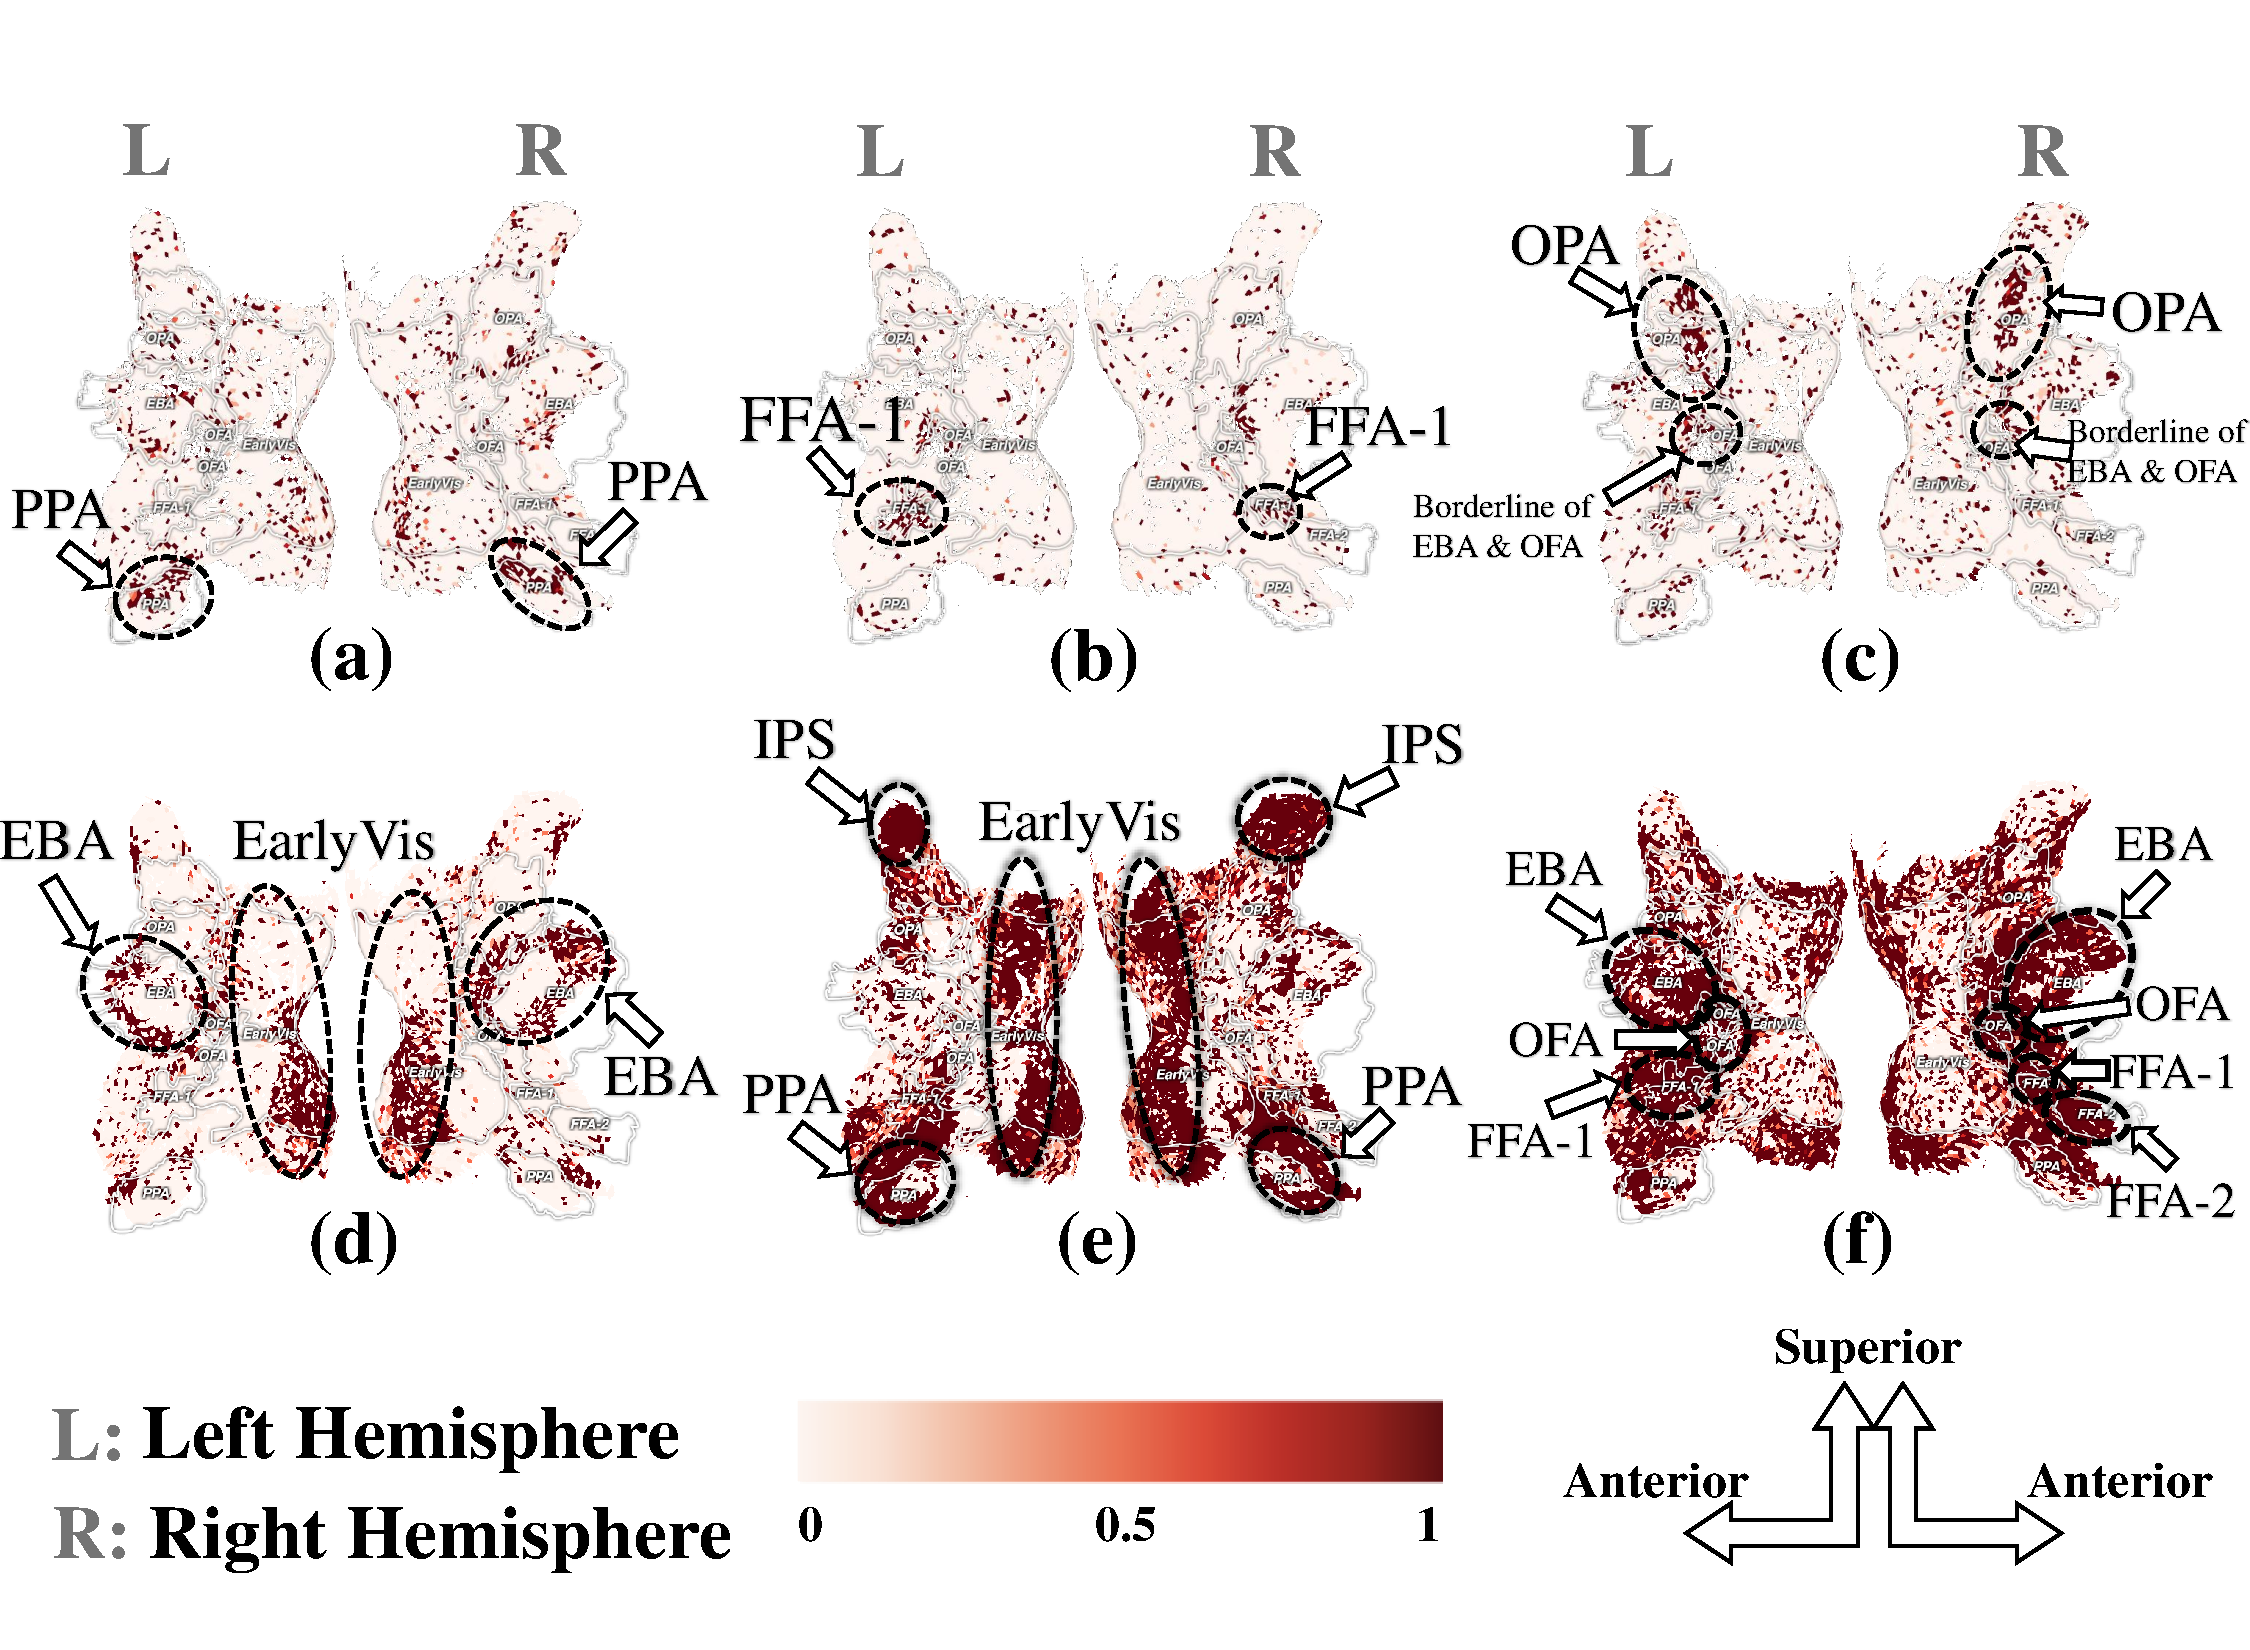
\includegraphics[width=\linewidth]{figures/brainmap.pdf}
    \caption{Each subfigure corresponds to a specific query of subject 1. We visualize the attention map between that query token and all voxels. Here we randomly select 6 query tokens, each of which exhibits a distinct spatial focus.}
    \label{fig:query}
\end{figure}


Unlike previous deep learning models \cite{scotti2024mindeye2,mai2023unibrain}, our model allows interpretations by investigating how \textit{queries} work in the neuroscience-informed attention layer. We inspect the attention weights between queries and voxels in Figure~\ref{fig:query}. 
% Weight values are scaled by min-max normalization and results are presented in Figure \ref{fig:query}. 

We found that some queries primarily focus on processing single brain regions, such as Parahippocampal Place Area (PPA) (Figure~\ref{fig:query}a) and Fusiform Face Area (FFA) (\ref{fig:query}b). As previous research has shown, PPA is related to conceptual association, semantic processing and environmental memory \cite{epstein1999parahippocampal,kohler2002differential,bar2008scenes,epstein2010reliable} and FFA is known for its critical role in expertise recognition, social cognition and identity memory \cite{schultz2003role,tsantani2021ffa,xu2005revisiting}. Both are important brain regions for the conceptualization of visual information and are responsible for the interaction between real-time stimulus and past memory \cite{brewer1998making,ranganath2004category,golarai2007differential}. 

Moreover, there are some queries that attend to multiple brain regions, revealing the information transmission between low- and high-level brain regions. For instance, interactions between early visual areas and higher-level regions like PPA and IntraParietal Sulcus (IPS) (Figure~\ref{fig:query}e), revealing a potential pattern for human attention-guided actions \cite{tunik2007beyond,connolly2016coding}. Additionally, queries are also found responsible for communications between high-level brain regions (Figure \ref{fig:query}c,\ref{fig:query}f). Together, these findings indicate that the learnable queries may reflect the dynamics of human brain activities in the visual task, from seeing and thinking about the image to pressing the button for the visual recall task in NSD \cite{allen2022massive}. 


We provide attention map visualizations of subjects other than subject 1 in Appendix~\ref{app:brainmap_other}. We also visualize latent embeddings during the model forward pass in Appendix~\ref{app:latent}. Qualitative analysis of model responses could be found in Appendix~\ref{app:qual}.
